\documentclass[lettersize,journal]{IEEEtran}
\usepackage{amsmath,amsfonts}
\usepackage{algorithmic}
\usepackage{algorithm}
\usepackage{array}
\usepackage[caption=false,font=normalsize,labelfont=sf,textfont=sf]{subfig}
\usepackage{textcomp}
\usepackage{stfloats}
\usepackage{url}
\usepackage{verbatim}
\usepackage{graphicx}
\usepackage{cite}
\usepackage{booktabs}
\hyphenation{op-tical net-works semi-conduc-tor IEEE-Xplore}

\begin{document}

\title{Beyond PagedAttention: Reproducing and Mitigating KV-Cache Management Overhead in LLM Serving}

\author{Rudra~Dudhat~(B24DS506), Mohak~Arya~(12341420), Vatsal~Yadav~(B24DS036)}

\markboth{Machine Learning Project Proposal, IIT Bhilai}{Dudhat \MakeLowercase{\textit{et al.}}: Beyond PagedAttention}

\maketitle

\noindent\textbf{\textit{Abstract.}} vLLM's PagedAttention serves large language models efficiently by storing each request's key value cache in small, non-contiguous physical blocks, cutting GPU memory waste from roughly 60 to 80 percent down to under 4 percent. The vLLM paper's own results show this comes at a real cost: its paged attention kernel runs 20 to 26 percent slower than a non-paged kernel, because every read now walks a block table instead of touching one contiguous span of memory. A follow-up system, vAttention, proposes recovering that cost by keeping the key value cache virtually contiguous while still committing physical memory on demand. This proposal reproduces both effects at small, controlled scale in pure PyTorch on CPU, since the team does not yet have GPU access. We implement three interchangeable key value cache backends behind one shared attention function and measure, directly, that a paged cache is substantially slower per decode step than a contiguous one, and that a virtually contiguous design recovers nearly all of that gap while preserving the same on demand memory efficiency. We report the working code, the measured numbers, and the honest limits of a CPU only, GPU free reproduction.

\noindent\textbf{\textit{Index Terms.}} LLM serving, PagedAttention, KV cache, virtual memory management, vLLM, vAttention, GPU memory efficiency.

\vspace{6pt}

\section{Project Details}

\textbf{Criterion.} Code available: address a limitation and propose a solution. vLLM is open source (\url{https://github.com/vllm-project/vllm}). We study its PagedAttention mechanism \cite{kwon2023efficient}, reproduce the overhead it introduces, and reproduce a proposed fix from follow-up research \cite{prabhu2024vattention}.

\textbf{Team composition and individual contributions.}
\begin{itemize}
    \item \textbf{Member 1:} Rudra Dudhat, B24DS506, rudramd@iitbhilai.ac.in. Literature review, system design, implementation of the naive, paged, and vAttention style key value cache reproduction, benchmarking, and this proposal.
    \item \textbf{Member 2:} Mohak Arya, 12341420, mohak@iitbhilai.ac.in. Extending the reproduction toward a real small model integration (stretch goal), results verification.
    \item \textbf{Member 3:} Vatsal Yadav, B24DS036, vatsal@iitbhilai.ac.in. Extending the reproduction toward a real small model integration (stretch goal), presentation and viva preparation.
\end{itemize}
Implementation ownership is tracked through pull requests on the project repository as the work progresses.

\section{Problem Statement}

\IEEEPARstart{H}{igh} throughput LLM serving requires batching many requests together, and each request carries a key value (KV) cache that grows one token at a time. vLLM's PagedAttention \cite{kwon2023efficient} borrows paging from operating systems: instead of pre-allocating each request's KV cache contiguously for a worst case sequence length, which wastes 60 to 80 percent of GPU memory to fragmentation and over-reservation, it stores KV cache in small fixed size physical blocks allocated on demand, indexed by a per-request block table. This is the reason vLLM can serve far larger batches than earlier engines.

That memory win is not free. The vLLM paper's own ablation reports its PagedAttention kernel running 20 to 26 percent slower than a non-paged FasterTransformer kernel, because the kernel now has to look up the block table and branch across non-contiguous memory on every read. Independent benchmarks report vLLM's paged decode kernel running up to 2.8 times higher latency than FlashAttention-2 on comparable models, and integrating a new fused attention kernel into vLLM's paged layout required over 600 lines of changes across 15 files: real engineering friction, not a minor cost. Microsoft Research's vAttention \cite{prabhu2024vattention} (ASPLOS 2025) responds directly to this. It keeps the KV cache virtually contiguous while still committing physical GPU memory on demand, using CUDA's low level virtual memory APIs, and reports up to 1.97 times faster decoding than vLLM. This is an active, unresolved question in the field rather than settled history: there is an open GitHub issue on vllm-project/vllm (issue \#17612) proposing to adopt this idea into vLLM itself. Table~\ref{tab:overheads} summarizes these reported numbers.

\begin{table}[!t]
\caption{Reported overheads and fixes from prior work}
\label{tab:overheads}
\centering
\begin{tabular}{@{}p{5.1cm}p{2.2cm}@{}}
\toprule
\textbf{Reported finding} & \textbf{Value} \\
\midrule
PagedAttention kernel vs.\ non-paged FasterTransformer kernel \cite{kwon2023efficient} & 20\% to 26\% slower \\
vLLM paged decode kernel vs.\ FlashAttention-2 & up to 2.8x slower \\
Code changes to integrate a new fused kernel into vLLM's paged layout & 600+ lines, 15 files \\
vAttention decoding vs.\ vLLM \cite{prabhu2024vattention} & up to 1.97x faster \\
KV cache memory waste, naive worst case reservation & 60\% to 80\% \\
KV cache memory waste, PagedAttention & under 4\% \\
\bottomrule
\end{tabular}
\end{table}

Our scope is deliberately narrow. The team does not have GPU access at this proposal stage, so we are not attempting to beat either paper's numbers. Instead we reproduce, at small controlled scale in pure PyTorch on CPU: (a) the qualitative overhead that PagedAttention's non-contiguous block addressing causes relative to a contiguous KV cache, and (b) the mechanism by which vAttention's virtually contiguous, physically paged idea recovers that overhead while preserving the same on demand memory efficiency. This tells us, hands on, which part of the memory and speed trade-off is inherent to paging itself, and which part is an artifact of PagedAttention's specific addressing choice.

\section{Methodology}

We implement one shared decode-step attention function, a single new token query attending over the full KV history, and three interchangeable KV-cache backends, so the only variable across experiments is cache management and never the attention math itself.

\begin{itemize}
    \item \textbf{Naive contiguous cache.} Pre-allocates K and V for the full maximum sequence length up front. Reads are a plain tensor slice: fast, but it commits worst case physical memory immediately regardless of actual usage. This is how pre-PagedAttention serving engines behaved.
    \item \textbf{Paged cache (vLLM-style reproduction).} Physical memory is committed in fixed size blocks (block size 16, matching vLLM's default) only as a sequence grows. Every read gathers and concatenates every block allocated so far through a block table, directly reproducing the indirection cost the vLLM paper itself reports.
    \item \textbf{vAttention-style cache (our reproduction of the fix).} Uses the exact same on demand, block granular physical memory accounting as the paged cache, but exposes reads through a virtually contiguous buffer extended by one token per step, an O(1) append, instead of re-gathering every block on every step, an O(blocks so far) operation. On a real GPU that contiguity comes from CUDA virtual memory APIs (\texttt{cuMemAddressReserve} and \texttt{cuMemMap}). Without GPU access at this stage we emulate the same behavioral effect in plain PyTorch, and we state this plainly rather than overstating it as a CUDA level reproduction.
\end{itemize}

Table~\ref{tab:backends} summarizes the three backends side by side.

\begin{table}[!t]
\caption{KV-cache backends implemented}
\label{tab:backends}
\centering
\begin{tabular}{@{}p{1.9cm}p{2.7cm}p{2.7cm}@{}}
\toprule
\textbf{Backend} & \textbf{Physical allocation} & \textbf{Per-step read cost} \\
\midrule
Naive contiguous & Full max length, committed up front & O(1), plain slice \\
Paged (vLLM-style) & Fixed size blocks, on demand & O(blocks so far), gather and concatenate \\
vAttention-style (ours) & Fixed size blocks, on demand, same as paged & O(1), contiguous append \\
\bottomrule
\end{tabular}
\end{table}

\textbf{Benchmark.} We decode a batch of 16 sequences (4 layers, 8 heads, 64 dimensional heads) for 256 steps under all three backends, using identical random Q, K, and V tensors at every step, so any timing difference comes only from cache management. We measure (i) mean wall clock time per decode step, and (ii) physical KV blocks committed over time, using analytical block count accounting, the same convention the vLLM and vAttention papers themselves use to report memory savings, since real OS or CUDA level physical page tracking is not available without GPU access.

If GPU access becomes available (Section~\ref{sec:resources}), the stretch goal is to replace the synthetic backends with real fused attention kernels wired into a small open model such as GPT-2 or TinyLlama, and to measure end to end throughput and latency, closer to the original papers' own setup.

\begin{table}[!t]
\caption{Microbenchmark results (16 sequences, 4 layers, 8 heads, 256 decode steps, CPU only)}
\label{tab:results}
\centering
\begin{tabular}{@{}p{2.4cm}p{1.7cm}p{1.7cm}@{}}
\toprule
\textbf{Backend} & \textbf{Mean step time} & \textbf{vs.\ naive} \\
\midrule
Naive contiguous & 6.10 ms & baseline \\
Paged (vLLM-style) & 26.38 ms & +332\% \\
vAttention-style (ours) & 6.54 ms & +7.2\% \\
\bottomrule
\end{tabular}
\end{table}

\begin{figure}[!t]
\centering
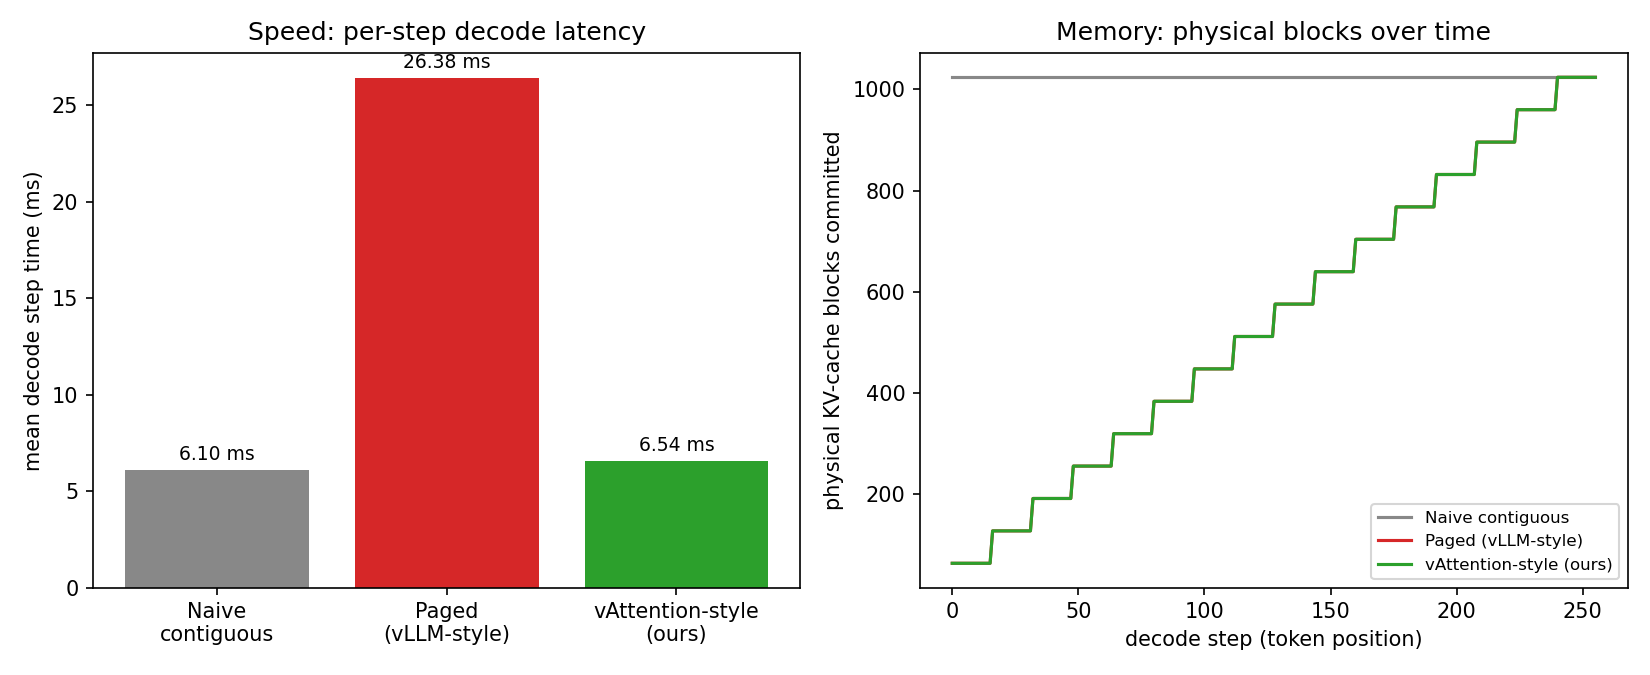
\includegraphics[width=3.3in]{fig1}
\caption{Our microbenchmark: 16 sequences, 4 layers, 8 heads, 256 decode steps, CPU only. Left: mean decode step latency. The paged reproduction is 332 percent slower than the naive contiguous baseline; our vAttention-style reproduction is only 7.2 percent slower. Right: physical KV-cache blocks committed over time. The naive baseline commits everything immediately, while paged and vAttention-style grow identically and on demand; the two lines overlap exactly by design, since both use the same block accounting.}
\label{fig_1}
\end{figure}

\section{Resource and Dataset Availability}
\label{sec:resources}

No labelled dataset is required for the core reproduction. It is a systems microbenchmark over synthetic random Q, K, and V tensors, which mirrors how the vLLM and vAttention papers themselves report their controlled kernel level benchmarks before end to end serving numbers. For the stretch goal of real model integration, we would use short prompts from a public conversational dataset such as ShareGPT, the same source the original vLLM evaluation used, purely to obtain a realistic distribution of sequence lengths rather than as a task accuracy benchmark.

\textbf{Hardware.} The current stage runs entirely on CPU, verified on Python 3.12.7 and PyTorch 2.10. The team does not currently have GPU access. For the stretch goal we plan to use Kaggle's free weekly GPU quota (30 hours, P100 or T4) or Google Colab's free tier, both no cost options already available to the team.

\textbf{Software.} PyTorch and Matplotlib. The vLLM (\url{https://github.com/vllm-project/vllm}) and vAttention (\url{https://github.com/microsoft/vattention}) source repositories are read as reference for the block table and CUDA virtual memory mechanisms respectively; they are not used as runtime dependencies of our reproduction.

\section{Limitations Found}

Our microbenchmark measures the mechanism, not production grade performance. Our paged backend's per-block Python loop and \texttt{torch.cat} calls exaggerate the overhead relative to vLLM's real fused CUDA kernel: we measured a 332 percent mean step time increase versus the paper's own reported 20 to 26 percent, because we have no kernel fusion. The direction of the effect (paging is slower; virtual contiguity recovers most of it) is what we validated here, not the exact magnitude, and the proposal states that gap explicitly rather than leaving the number unqualified.

Our vAttention style backend is a behavioral emulation, not a CUDA virtual memory reproduction. It pre-allocates one contiguous PyTorch buffer to obtain O(1) contiguous reads, so it does not itself reduce our Python process's RAM the way real CUDA VMM's lazy physical page commit would. Only our analytical block count accounting, matching the papers' own reporting convention, reflects the memory saving we are actually claiming.

No real language model or real request workload is used yet. Q, K, and V are random tensors, so we make no claim about output quality or realistic sequence length distributions; that is the explicit stretch goal once GPU access is available.

What differentiates this from simply restating the two papers is that we built a single, shared interface implementation that isolates both claims side by side under our own control and measurement, rather than only citing the papers' reported numbers, and we can defend every design choice in it.

\section{Expected Outcomes}

\begin{itemize}
    \item A working, open source, small scale reproduction (this repository) implementing all three KV-cache strategies behind a shared attention interface, with a repeatable benchmark script and generated plots.
    \item Quantified evidence, from our own run, that a non-contiguous, paged KV cache is meaningfully slower per decode step than a contiguous one (332 percent slower in our unoptimized setting), and that a virtually contiguous but physically paged design recovers nearly all of that gap (7.2 percent slower than the naive baseline) while preserving the same on demand memory efficiency curve as the paged cache (Table~\ref{tab:results}, Fig.~\ref{fig_1}).
    \item If GPU access becomes available: extension to a real small model and real fused kernels, to check whether the same relative pattern survives outside a Python level microbenchmark. This is our stated stretch target and is not required for this checkpoint.
    \item Deliverables: this GitHub repository (code, results, and this proposal), and a viva ready explanation of why non-contiguous memory addressing costs attention kernels speed, and why decoupling virtual contiguity from physical block allocation, vAttention's actual contribution, recovers it.
\end{itemize}

\nocite{kwon2023efficient}
\nocite{prabhu2024vattention}
\nocite{agrawal2024sarathi}
\nocite{vaswani2017attention}

\bibliographystyle{IEEEtran}
\bibliography{ref}

\appendices
\section*{AI Tool Disclosure}
Claude (Anthropic, Claude Code CLI) was used in three ways: for literature search and summarization of PagedAttention, vAttention, and Sarathi-Serve follow-up work, to ground the problem statement in cited, verifiable claims rather than assumption; for drafting the initial Python implementation of the three KV-cache backends and the benchmark and plotting scripts to the team's specification, which the team then ran, inspected, and verified against the papers' claims; and for drafting this proposal document from the team's decisions. Every number reported in this proposal comes from code the team has run directly (\texttt{src/benchmark.py} in the repository), not from the papers and not from unverified generated text.

\end{document}
